\chapter{Data Reduction and Analysis}
	\label{cha:Data}

From this point on, the two datasets are treated almost identically. The only difference (other than the different spectral range and resolutions) is that the MUSE datacubes were binned to a higher signal to noise ratio (S/N).

\section{VIMOS data}
	\label{sec:VIMOS}

\section{MUSE data}
	\label{sec:MUSE}


\section{Data Analysis}
	\label{sec:analysis}
	Given that galaxy (the signal) is brightest at the center and fades away radially, while the noise, which is assumed to be Poisson dominated scales as the square root of the signal, the S/N will be highest at the center, decreasing with increasing radius. In the out regions of a galaxy, it becomes too low for to make meaningful fits to the spectra. Because of this we spatial bin to a set S/N (increasing a bins size until it reaches the require S/N). We do this using a Voronoi Binning routine\footnote{\textsc{IDL} and \textsc{Python} routines for \textsc{voronoi\_2d\_binning} can be found at http://www-astro.physics.ox.ac.uk/~mxc/software/} by \citet{Cappellari2003}. This  which is fast becoming an 'industry standard' method for adaptive 2D binning. To do this, we defined 'signal' and 'noise' as the median value of the spectrum and noise spectrum respectively for each spaxel, and required a target S/N of 30 for all VIMOS datacubes, 50 for IC 1459 and IC 4296 MUSE datacubes and 100 for NGC 1316 and NGC 1399 datacubes. The MUSE datacubes had differing S/N due to the sky subtractions that were applied. These were successful in removing artifacts from the spectra of IC 1459 and IC 4296 which allowed us to retain a higher level of spatial information (by binning to a lower S/N) for these two galaxy. Unfortunate they were not appropriate for the observations of NGC 1316 and NGC 1399 due to the angular size of these objects and the tessellated nature of the their observations (see section \ref{sec:skysubtractions}). Figure \ref{fig:egSNR} shows an example of the S/N of the bins. In it, concentric ringed structures can be clearly seen around the center of the galaxy as bins with a S/N just below to target are increased in size by a single spaxel meaning they have a final S/N well over the target.

	% Need to remove bin numbers, galaxy name and redshift and second axis from plot.
	\begin{figure}
		\centering
		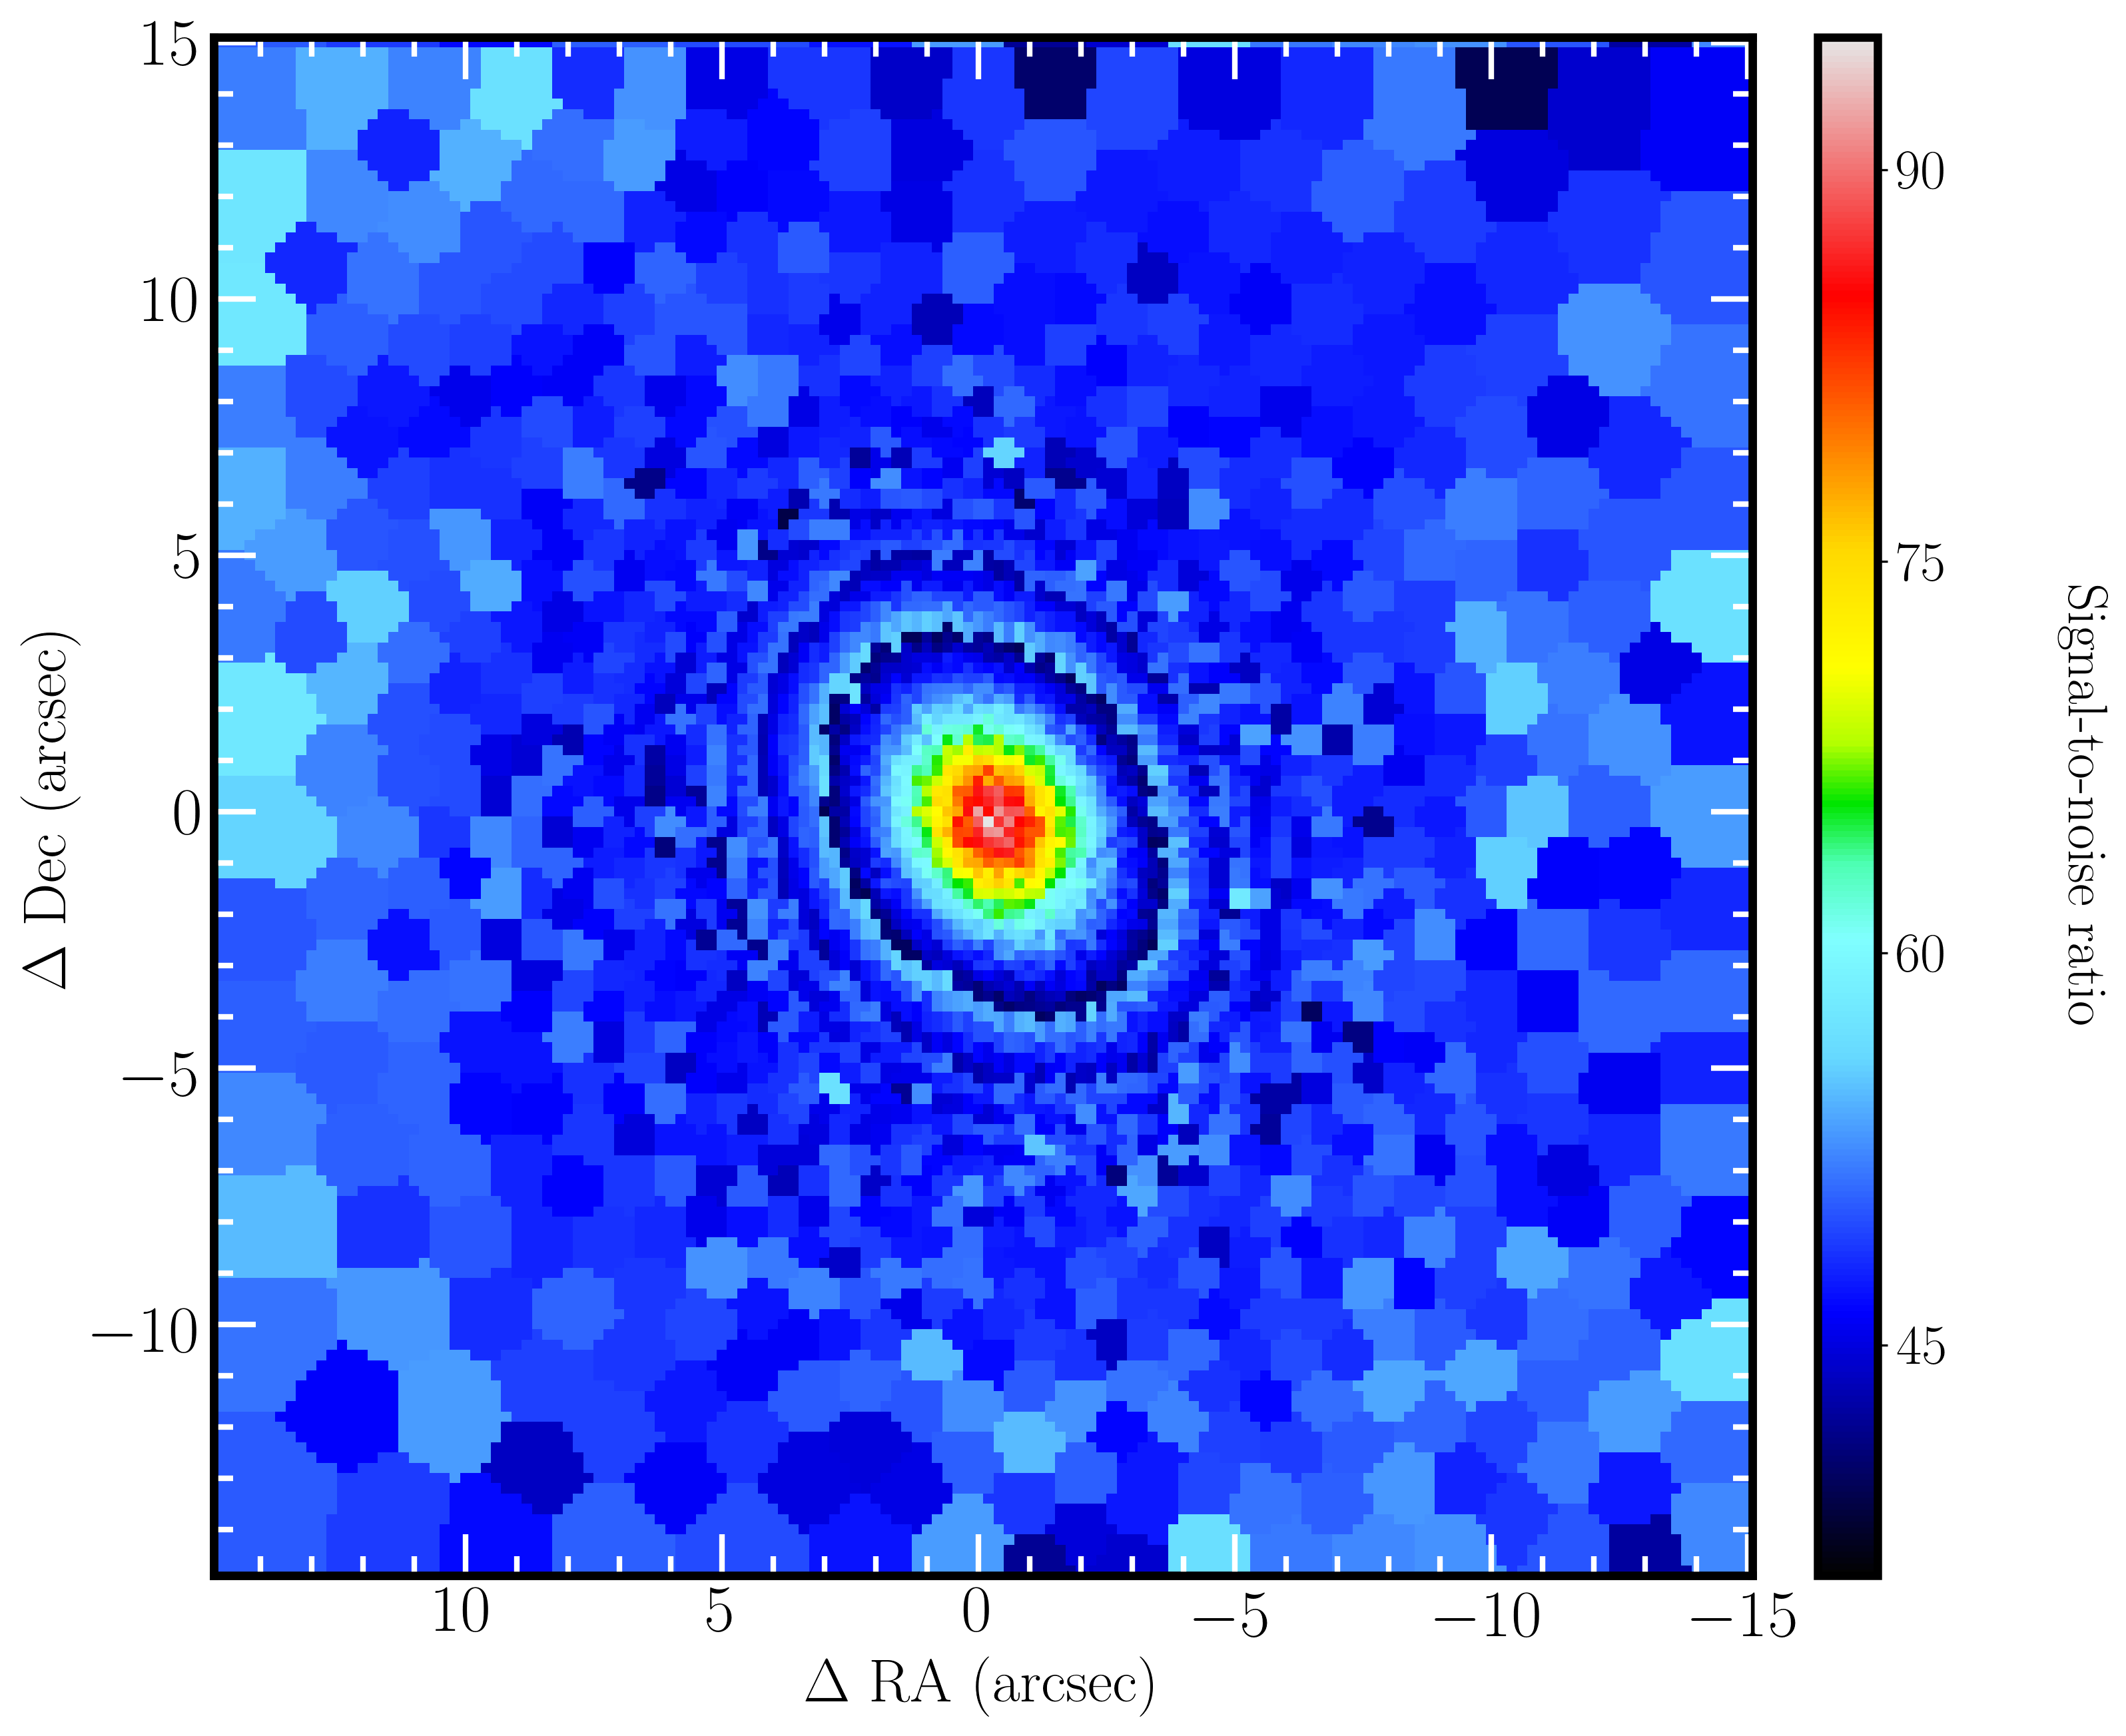
\includegraphics[width=.6\textwidth]{chapter2/egSNR.png}
		\caption[Example S/N map]{The figure shows an example S/N map (color scale) for the MUSE observation of IC 1459. The flux contours are shown in black.}
		\label{fig:MassRe}
	\end{figure}


	Our analysis makes use of the penalized-fitting routine \textsc{ppxf}\footnote{\textsc{IDL} and \textsc{Python} routines for \textsc{ppxf} can be found at http://www-astro.physics.ox.ac.uk/~mxc/software/} by \citet{Cappellari2004, Cappellari2016a}. This routine finds the bestfitting spectra by building galactic spectra from combined stellar templates and convolving them with a Gaussian line-of-sight velocity distribution (LOSVD, we did not allow any deviations from a Gaussian profile for the stellar fits). Additive and multiplicative corrections to the continuum level can also be included in the fit using Lagrange polynomials. Regions (800 km s$^-1$ wide) around possible emission lines were masked. Emission lines included were: [OII]3726 , [OII]3729, H$_\delta$, H$_\gamma$, H$_\beta$, [OIII]4959, [OIII]5007, [NI]5199, [NI]5202, [OI]6300, [OI]6364, [NII]6548, [NII]6583, H$_\alpha$, [SII]6716 and [SII]6731. A telluric line at 5199\AA, seen in some of the VIMOS spectra, was also masked, though the exact location of this depended on the initial redshift 'guess' since the spectrum is moved to the rest frame of the galaxy. For this analysis, we also allowed an additive continuum correction using a fourth order Lagrange polynomial.

	In order to improve the speed of our analysis, we first collapse the datacube spatially to give global spectra for the galaxy. Obviously this means that the contribution from each spaxel is weight by its luminosity. Then the entire Miles stellar library \citep{} is used as templates for \textsc{ppxf} to fit. For our 14 datacubes (10 VIMOS and 4 MUSE), this step fits an average of \_\_\_\_\_\_ out of 985 templates with a weighting of zero. When a template for a particular datacube is given a zero weighting at this step it is not used for future analysis of that datacube. This drastically improves the runtime of \textsc{ppxf} without effecting the quality of the fit. For this fit the redshift from Simbad is used to move the spectra to the rest frame such that an initial guess of the velocity within that frame is 0 km s$^{-1}$. We use a initial guess of the velocity dispersion of 200 km s$^{-1}$ since ETGs have dispersions of around this value and higher. 

	Next we run a very simply Markov chain Monte Carlo (MCMC) routine to find more optimum initial guesses for velocity and velocity dispersion. The initial run is set up in the same way as the previous step (though only using the templates with non-zero weightings). After each run, the fitted velocity and velocity dispersion were used to iteratively improve the initial guess for the next run. After the first three reps, the velocity was used to calculate the redshift of the galaxy: these are the redshift values quoted in \ref{tab:sample}. After this 100 reps were run with the mean velocity (in the de-redshifted frame) and velocity dispersion were recorded and used as the initial guesses for all fits in that datacube. 

	Beyond this point, each bin is analyzed independently. Each one is processed through \textsc{ppxf} using only the Miles templates with non-zero weighting from above, using the redshift, additional velocity and dispersion estimates from the last step. 







	The entire pipeline summed up is as follows:
	\begin{enumerate}
		\item Spatial bin using Voronoi binning
		\item Find relevant stellar templates by fitting the entire galaxy spectra with all the templates from the Miles library
		\item Estimate redshifts and global line-of-sight velocity dispersion with MCMC routine 
		\item Find bestfitting LOSVD for each individual bin
		\item Use bootstrapping method to estimate uncertainties LOSVD measurements. 
	\end{enumerate}

